\chapter{Proposta}
\label{ch:proposta}

A proposta principal deste trabalho é de desenvolver uma versão do algoritmo FSS aplicando em problemas dinâmicos com domínio contínuo, de forma que os operadores evolutivos que foram estudados neste trabalho possam ser aplicados e/ou adaptados nessa versão do FSS. Além dos operadores será aplicado as técnicas de manutenção da diversidade populacional estudadas neste trabalho. O algoritmo final terá a possibilidade de alternar nos operadores evolutivos, de modo que cada operador possa ser analisado individualmente (aplicado do FSS) ou em conjunto com outro operador e/ou técnica de manutenção de diversidade populacional. uma aplicação do tipo é a versão híbrida do PSO com o FSS, porém nesse caso os operadores do FSS que foram aplicados no PSO \cite{cavalcanti2011hybrid}.

Com este algoritmo será possível realizar experimentos para validar a relevância dos operadores utilizados para cada classe de problemas. Além disso será possível analisar a interação dos operadores entre si e entre as técnicas de manutenção da diversidade populacional.

Para a realização dos testes serão aplicadas as mesmas métricas de performance, satisfabilidade, robustez e diversidade para realizar uma comparação justa e detalhada dos componentes usados no algoritmo final

\section{Estudo de Caso}
\label{sec:test_case}

Nos testes foram feitas 30 aplicações para cada função, utilizando: 30 dimensões, 30 peixes e 5.000 iterações sendo que o o número total de avaliações de \textit{fitness} é de 300.000.

\begin{table}[]
\centering
\caption{My caption}
\label{my-label}
\begin{tabular}{l}
\begin{figure}
	\caption{Representação gráfica da influência do Movimento Coletivo Instintivo de uma contração}
	\centering
	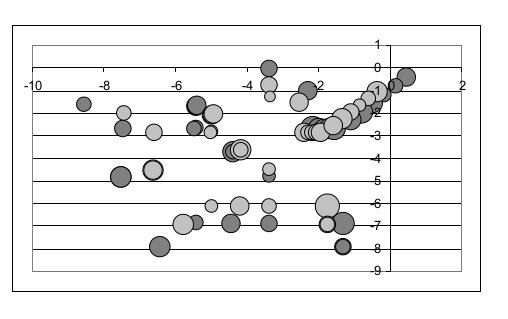
\includegraphics[scale=0.5]{images/movimento_volatil.png}
\end{figure} 
\end{tabular}
\end{table}